\chapter{本书内容的基本环境配置}
本书是目标是介绍一个AI换脸系统的开发流程,主要是讲解整个系统的整体结构、流程,核心算法及加速算法。并附带完整代码的Git地址。读者学完后可以开发这个系统作为基础,有想法的读者可以进行扩充,就可以开发一个商业软件。
我使用的开发环境是操作系统是wsl,即在windows10 系统上安装了Ubuntu 22.04子系统,具体安装方法,可以自行查阅相关资料。
首先安装的开发工具CUDA,我选的版本是11.8,不算特别新,也不算特别古老。适合于当前流行的Nvida显卡。同时安装的CUDNN,这是神经网络的开发库。具体安装方法可以参考\url{https://gist.github.com/MihailCosmin/affa6b1b71b43787e9228c25fe15aeba?permalink_comment_id=4850089}。演示了CUDA和CUDNN的安装及验证代码。
TensorRT 是 NVIDIA 推出的用于深度学习推理加速的高性能推理引擎。它可以将深度学习模型优化并部署到 NVIDIA GPU 上,实现低延迟、高吞吐量的推理过程。TensorRT 主要用于加速实时推理任务,如物体检测、图像分类、自然语言处理等。
所需的库是:
\begin{itemize}
\item \textbf{CUDA}
\item \textbf{TensorRT}
\item \textbf{OpenCV}:

下面就逐一讲解每个库的安装方法,

1.安装CUDA
我们选择安装的CUDA版本是11.8。它是一个比较通用的版本。
安装过程如下:
\begin{lstlisting}{c}
     mkdir Downloads && cd Downloads #为了模仿Ubuntu系统,我们自己创建了Downloads文件夹,用来存储下载的文件。
     sudo apt update && sudo apt upgrade -y #更新一些库
     sudo apt install g++ freeglut3-dev build-essential libx11-dev libxmu-dev libxi-dev libglu1-mesa libglu1-mesa-dev #安装所需的依赖库
     sudo wget https://developer.download.nvidia.com/compute/cuda/repos/ubuntu2204/x86_64/cuda-ubuntu2204.pin #   APT 软件包优先级配置文件,确保系统从正确的仓库(如 NVIDIA 官方仓库)安装 CUDA 工具包
     sudo mv cuda-ubuntu2204.pin /etc/apt/preferences.d/cuda-repository-pin-600 #移动到/etc/apt路径下 
     sudo apt-key adv --fetch-keys https://developer.download.nvidia.com/compute/cuda/repos/ubuntu2204/x86_64/3bf863cc.pub #这是一个 GPG 公钥文件,用于验证从 NVIDIA CUDA 仓库下载的软件包的签名,确保其完整性和来源可信。 
     sudo add-apt-repository "deb https://developer.download.nvidia.com/compute/cuda/repos/ubuntu2204/x86_64/ /" 
     sudo apt install cuda-11-8 -y   
     echo 'export PATH=/usr/local/cuda-11.8/bin:$PATH' >> ~/.bashrc  
     echo 'export LD_LIBRARY_PATH=/usr/local/cuda-11.8/lib64:$LD_LIBRARY_PATH' >> ~/.bashrc 
     source ~/.bashrc 
     sudo ldconfig
     nvcc -V #查看安装结果,如果显示 "Cuda compilation tools, release 11.8, V11.8.89" 表示安装成功了。
\end{lstlisting}
接着还要安装一下 CUDNN库。下面指令仍然是在~/Downloads路径下面执行。
\begin{lstlisting}{c}
    CUDNN_TAR_FILE="cudnn-linux-x86_64-8.7.0.84_cuda11-archive.tar.xz" 
    sudo wget https://developer.download.nvidia.com/compute/redist/cudnn/v8.7.0/local_installers/11.8/cudnn-linux-x86_64-8.7.0.84_cuda11-archive.tar.xz  
    sudo tar -xvf ${CUDNN_TAR_FILE} 
    sudo tar -xvf ${CUDNN_TAR_FILE}  #解压
    sudo mv cudnn-linux-x86_64-8.7.0.84_cuda11-archive cuda
    sudo cp -P cuda/include/cudnn*.h /usr/local/cuda-11.8/include   
    sudo cp -P cuda/lib/libcudnn* /usr/local/cuda-11.8/lib64/                                                                 
    sudo chmod a+r /usr/local/cuda-11.8/lib64/libcudnn*
\end{lstlisting}
查看CUDNN的版本,执行如下命令
\begin{lstlisting}{c}
    cat /usr/local/cuda/include/cudnn_version.h | grep CUDNN_MAJOR -A 2
\end{lstlisting}

我主要参考这个网页\url{https://gist.github.com/MihailCosmin/affa6b1b71b43787e9228c25fe15aeba?permalink_comment_id=4850089}。

2. 安装TensorRT
 安装TensorRT比较简单,就是下载库文件,解压,设置环境变量即可。
 \begin{lstlisting}{c}
 #下载到 ~/Downloads
 cd ~/Downloads
 wget https://developer.nvidia.com/downloads/compute/machine-learning/tensorrt/secure/8.6.1/tars/TensorRT-8.6.1.6.Linux.x86_64-gnu.cuda-11.8.tar.gz
 #解压到  /usr/local/
sudo tar -xzvf TensorRT-8.6.1.6.Linux.x86_64-gnu.cuda-11.8.tar.gz -C /usr/local/
   
 \end{lstlisting}
 设置环境变量
 \begin{lstlisting}
    
 sudo vim ~/.bashrc
 export LD_LIBRARY_PATH=/path/to/tensorrt/lib:$LD_LIBRARY_PATH
 export LD_LIBRARY_PATH=/usr/local/TensorRT-8.6.1.6/lib:$LD_LIBRARY_PATH
 source ~/.bashrc
 \end{lstlisting}


3. 安装OpenCV(CUDA版)

OpenCV是出来图片的基础库,我们使用CUDA版本,有利于加速。
步骤如下:
\begin{listing}
 sudo apt update
 sudo apt upgrade                
 sudo apt install build-essential cmake pkg-config unzip yasm git checkinstall       
 sudo apt install libjpeg-dev libpng-dev libtiff-dev           
 sudo apt install libavcodec-dev libavformat-dev libswscale-dev         
 sudo apt install libgstreamer1.0-dev libgstreamer-plugins-base1.0-dev                              
 sudo apt install libxvidcore-dev libx264-dev libmp3lame-dev libopus-dev                                                 
 sudo apt install libmp3lame-dev libvorbis-dev                                                                            
 sudo apt install ffmpeg                                        
 sudo apt install libva-dev  
 sudo apt install libdc1394-25 libdc1394-dev libxine2-dev libv4l-dev v4l-utils                                          
 sudo ln -s /usr/include/libv4l1-videodev.h /usr/include/linux/videodev.h               
 sudo apt-get install libgtk-3-dev
 sudo apt-get install libtbb-dev  
 sudo apt-get install libatlas-base-dev gfortran   
 sudo apt-get install libprotobuf-dev protobuf-compiler
 sudo apt-get install libgoogle-glog-dev libgflags-dev 
 sudo apt-get install libgphoto2-dev libeigen3-dev libhdf5-dev doxygen  
 #进入~/Downloads目录下载Opencv源码并进行编译

 cd ~/Downloads && mkdir opencv && cd opencv
 wget -O opencv.zip https://github.com/opencv/opencv/archive/refs/tags/4.10.0.zip
 wget -O opencv_contrib.zip https://github.com/opencv/opencv_contrib/archive/refs/tags/4.10.0.zip
 unzip opencv.zip
 unzip opencv_contrib.zip
 cd opencv-4.10.0
 mkdir build
 cd build

 cmake -D CMAKE_BUILD_TYPE=RELEASE -D CMAKE_INSTALL_PREFIX=/usr/local -D WITH_TBB=ON -D ENABLE_FAST_MATH=1 -D CUDA_FAST_MATH=1 -D WITH_CUBLAS=1 -D WITH_CUDA=ON -D BUILD_opencv_cudacodec=OFF -D WITH_CUDNN=ON -D OPENCV_DNN_CUDA=ON -D CUDA_ARCH_BIN=7.5 
 -D WITH_V4L=ON -D WITH_QT=OFF -D WITH_OPENGL=ON -D WITH_GSTREAMER=ON -D OPENCV_GENERATE_PKGCONFIG=ON -D OPENCV_PC_FILE_NAME=opencv.pc -D OPENCV_ENABLE_NONFREE=ON -D OPENCV_EXTRA_MODULES_PATH=/home/an/Downloads/opencv/opencv_contrib-4.10.0/modules -D INSTALL_PYTHON_EXAMPLES=OFF -D INSTALL_C_EXAMPLES=OFF -D BUILD_EXAMPLES=OFF  ..
 # 编译安装
 nproc
  make -j8
  sudo make install

\end{listing}

其他的几个辅助库,它们有:

fmt 库是 C++ 中格式化输出的现代解决方案,提供了类型安全、易用性和高性能。fmt 库比传统 sprintf 和 iostream 更快:
安装方法:
\begin{listing}{c}
    git clone https://github.com/fmtlib/fmt.git
    cd fmt
    mkdir build
    cd build
    cmake ..
    make -j8
    sudo make install    
\end{listing}

然后再cmakelists补上fmt的include和lib
\begin{listing}{c}
    find_package(FMT REQUIRED)
    target_link_libraries(xxx  fmt::fmt)
\end{listing}


spdlog
spdlog 是一个快速的 C++ 日志库,具有高性能、易用性和丰富的功能特性。 spdlog 是 header-only 的,可以直接下载并包含头文件:#include "spdlog/spdlog.h"
下载、编译源码:
\begin{listing}
    git clone https://github.com/gabime/spdlog.git
    cd spdlog && mkdir build && cd build
    cmake ..  && make -j16
\end{listing}



一个实例。
在安装了这些库之后,我们可以举例子演示一下使用方法。参数项目的github网址如下。
参考项目网址 \url{https://github.com/cyrusbehr/tensorrt-cpp-api}
主要演示的功能如下:
\item \textbf{如何生成TensorRT engine 文件}
\item \textbf{如何声明一个简单的优化简表}
\item \textbf{推理精度}
\item \textbf{如何读写GPU显存}
\item \textbf{如何处理单个或者多个输入/输出}

首先看一下简单流程:\begin{figure}[H]
    \centering
    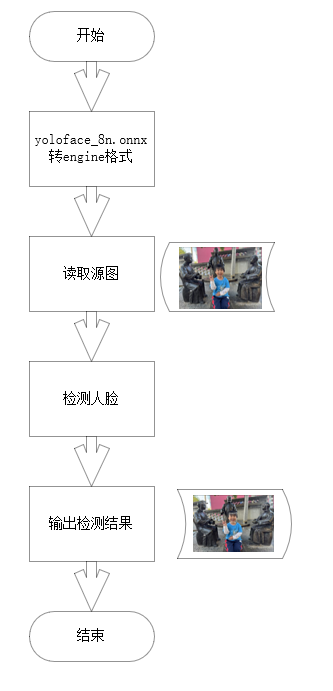
\includegraphics{figures/progress.png}
    \caption{Title of picture}
    \end{figure}





\begin{itemize}
\item \textbf{套装发行版:}俗称\LaTeX 的核心,常见的有CTeX套装、TeXlive套装(作者使用)、MacTeX套装等等,本文使用TeXlive2018版本,下载地址为\url{http://www.latexstudio.net/texsoftware}。

\item \textbf{编译引擎:}也是编译时点的按钮,本文采用魔法注释设置了编译引擎为xelatex,也是中文文档排版常用的编译引擎,其他的编译引擎有pdflatex、latex、bibtex等等。
 
\item \textbf{编辑器:}顾名思义,编辑器就是编辑tex文档所用的软件,编写本文档使用的是TeXstudio,也是作者推荐的一款编辑器,网上可以免费下载。下载tl2018时也会自带编辑器,名为TeXwork,也是一款很好的编辑器,编辑器的种类很多,甚至于word都可以拿来写tex代码,只不过tex编辑器拥有自带的语法高亮、自动补全等快捷方式。
\end{itemize}

\textbf{阅读或使用本模板时建议与tex文档对比学习。}

\section{文件结构}
解压压缩包后,内含的文件内容与结构如下
\begin{itemize}
\item \textbf{样本.pdf}:本文件,内包括写作方法与注意事项;
\item \textbf{CDUT\_ Lab\_ report.tex}:实验报告主文件,包括报告整体结构与一些全局定义;
\item \textbf{attachment文件夹}:内含文件attachment.pdf与attachment.docx,为实验报告中的心得体会,具体书写方式详见文末心得体会处;
\item \textbf{body文件夹}:内含各章节tex文档(如section\_1.tex),方便起见,每一章(每一实验)单独使用一个文档书写;
\item \textbf{figure文件夹}:文档中各类图片依照命名规范至于此文件夹中,方便统一管理,其中CDUT.png为文档必须图片,请勿删除;
\item \textbf{preface文件夹}:内含文档cover.tex为首页封面与目录设置;
\item \textbf{setup文件夹}:内含文档format.tex与package.tex,分别为全局设置文档与宏包文档,模板使用了模板必须与一些常用宏包,如有特殊需要可以自行添加在文档内,方便统一管理;
\item \textbf{texclear.bat}:用于清理辅助文件。
\end{itemize}

\section{由onnx到engine}
换脸的基础动作就是检测到人脸。对源图和目标图首先检测到人脸才能交换其特征,然后才能进行相关处理。
第一个网络就是使用Yolo网络进行人脸检测。
yoloface_8n.onnx 是一个轻量级人脸检测模型,属于 YOLO(You Only Look Once)系列模型的变种,专为高效人脸检测任务设计。
用于快速检测图像或视频帧中的多个人脸,并输出人脸的边界框(Bounding Box)及置信度。实行单阶段检测:类似 YOLO,直接回归边界框和类别,无需区域提议(RPN)。

可使用 Netron 工具可视化 .onnx 文件,直接查看输入/输出层名称和维度。
下图是 Netron截图的输入输出部分:
\begin{figure}[H]
\centering
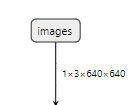
\includegraphics{figures/inputs.png}
\caption{Title of picture}
\end{figure}

\begin{figure}[H]
\centering
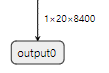
\includegraphics{figures/output.png}
\caption{Title of picture}
\end{figure}

我们设计了一个类,用来处理onnx转成engine格式,并且处理图片,检测人脸。
类图如下:\begin{figure}[H]
    \centering
    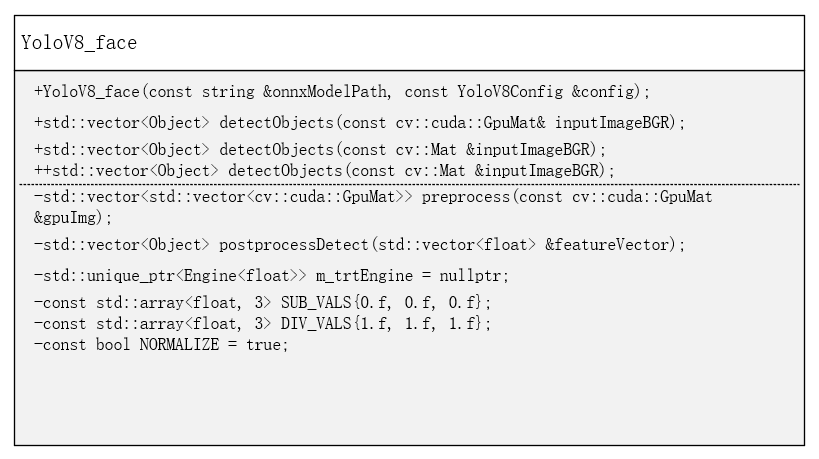
\includegraphics{figures/YoloV8_face.png}
    \caption{Title of picture}
    \end{figure}

类说明:
类名:YoloV8_face
功能:对模型进行格式转换,从.onnx 转为.engine格式文件。

成员函数:+YoloV8_face(const string &onnxModelPath, const YoloV8Config &config)
功能:构造函数,将onnx转为.engine文件。参数&onnxModelPath表示onnx文件, 参数config表示配置信息。

